\documentclass[dvipdfmx]{ehis}
\usepackage{graphicx}

\usepackage{amsmath,amssymb,amsfonts}
\usepackage{algorithmic}
\usepackage{textcomp}
\usepackage{xcolor}
\usepackage{url}
\usepackage{booktabs}
\usepackage[caption=false]{subfig}
\usepackage{multirow}
\usepackage{algorithm}
\usepackage{algorithmic}
\usepackage{listings}
\lstdefinelanguage{JavaScript}{
  keywords={const, let, var, function, return, if, else, for, while, switch, case, break, try, catch, finally, window, camerala_logger},
  sensitive=true,
  comment=[l]{//},
  morecomment=[s]{/*}{*/},
  morestring=[b]\",
  morestring=[b]\'
}
\lstdefinelanguage{csv}{
  morecomment=[l]{\#},
}

\newcommand{\etal}{\textit{et al.}}
\newcommand{\ie}{\textit{i.e.}}
\newcommand{\eg}{\textit{e.g.}}

\etitle{Camerala: A Browser-Native Framework for Task-Aligned Physiological Feature Logging in Home and Laboratory Settings}

\eauthor{
Kotaro Furukawa\thanks{College of Transdisciplinary Sciences for Innovation, Kanazawa University, Japan}
}

\YEAR{}
\VOL{}
\NO{}
\TYPE{}


\lstset{
  basicstyle=\ttfamily\scriptsize,
  breaklines=true,
  columns=fullflexible,
  keepspaces=true
}
\makeatletter
\def\@oddhead{}
\def\@evenhead{}
\def\ps@vr{
 \def\@oddhead{}
 \def\@evenhead{}
}
\def\ps@his{
 \def\@oddhead{}
 \def\@evenhead{}
}
\makeatother

\begin{document}

\begin{abstract}
Remote psychophysical experiments increasingly require methods for synchronizing behavioral task events with webcam-derived features while limiting the handling of privacy-sensitive video.
We present Camerala, a browser-native, local-first framework that integrates psychophysical task execution, on-device rPPG/FaceMesh-derived feature extraction, frame-level measurement-quality indicators, and timestamped local logging within a unified client-side runtime.
The framework avoids raw video transmission and, in the present implementation, stores extracted features and task events locally as CSV files packaged in a ZIP archive.
We evaluated Camerala in an exploratory 10-session deployment with one author-participant across one laboratory setting and one home setting.
The deployment completed under the tested configuration and produced synchronized task events, sensor-derived features, and measurement-quality indicators.
Descriptive results showed differences between the laboratory and home contexts in luminance, exposure fluctuation, face-tracking availability, head motion, and rPPG-oriented ROI estimates.
Because the study did not include reference physiological measurements, multiple participants, multiple devices, or controlled separation of environmental and task-related factors, these differences should be interpreted as deployment-specific sensor-derived observations rather than evidence of physiological, cognitive, psychological, or motivational effects.
The paper contributes a browser-native implementation example and design considerations for task-aligned, local-first physiological feature logging under limited home/laboratory conditions.
\end{abstract}

\begin{keyword}
Browser-Native Sensing, Remote Photoplethysmography, FaceMesh, Local-First Logging, Task-Aligned Measurement, Home/Laboratory Deployment
\end{keyword}

\maketitle

% =================================================================================
% SECTION 1: INTRODUCTION
% =================================================================================
\section{Introduction}

Remote or home-based psychophysical experiments often require synchronized behavioral task logs and webcam-derived features while avoiding unnecessary handling of privacy-sensitive video.
This use case differs from unconstrained daily-life sensing: the participant is expected to sit in front of a laptop, view task stimuli, and respond through the browser.
Even in this task-constrained setting, deployment outside a controlled laboratory introduces practical difficulties for human-interface research, including heterogeneous illumination, camera placement, posture, browser timing, and local data handling.

Many video-based physiological measurement pipelines rely on raw video recording or server-side processing.
Such approaches can be difficult to deploy in private spaces because raw facial video is privacy-sensitive and may be identifiable.
A local-first browser architecture offers an architectural privacy advantage: raw frames can be processed on the client device, while only extracted features, task events, and quality indicators are stored.
This does not constitute a dedicated privacy-preserving algorithm; rather, it is a system-design choice that reduces the need to transmit or retain raw video.

Real-time processing is treated here as a design choice for local-first feature logging rather than as the only technically possible architecture.
Recording video locally and processing it offline could preserve timestamps, but it would require storing privacy-sensitive raw video.
Camerala instead extracts features and quality indicators during task execution, allowing task events and sensing frames to be logged within the same client-side runtime without raw video persistence.
This design also supports online quality checks, such as detecting face-tracking failure, approximate face-size changes, and luminance instability during data collection.

To address this deployment scenario, we present \textbf{Camerala}, a browser-native framework for task-aligned physiological feature logging in task-constrained home/laboratory experiments.

\subsection{Research Questions}
We reformulated the exploratory Research Questions (RQs) to focus on operational completion and measurement-quality observations under the tested configuration:
\begin{itemize}
    \item \textbf{RQ1:} Under the tested laptop, browser, camera, and task configuration, can Camerala complete a task-constrained home/laboratory deployment while locally logging synchronized task events, sensor-derived features, and measurement-quality indicators without raw video transmission?
    \item \textbf{RQ2:} What descriptive differences in measurement-quality indicators and sensor-derived estimates are observed between the laboratory and home deployment contexts?
\end{itemize}

For RQ1, we used the following observation criteria: completion of the planned sessions and trials, local persistence of exported logs, synchronization of task events and frame-level feature logs, retention rate after predefined exclusion criteria, and availability of FPS, face size, face-tracking availability, luminance, exposure fluctuation, head motion, and rPPG-oriented ROI estimates.
These criteria are intended only to describe operational completion under the tested configuration; they do not demonstrate general deployability across users, devices, or environments.

\subsection{Contributions}
In this paper, we focus on system integration and conservative deployment observations. The contributions are:

\begin{enumerate}
    \item \textbf{Browser-native local-first sensing architecture}: A client-side pipeline that extracts rPPG/FaceMesh-derived features and measurement-quality indicators without transmitting or storing raw video.
    \item \textbf{Task-aligned on-device sensing and local persistence}: A unified browser runtime that synchronizes psychophysical task events with frame-level sensor-derived features and stores timestamped local logs.
    \item \textbf{Exploratory task-constrained home/laboratory deployment}: A limited N=1 author-participant deployment that illustrates operational completion and documents descriptive measurement-quality differences across the tested laboratory and home contexts.
\end{enumerate}

The remainder of this paper is organized as follows.
Section II reviews related work in rPPG, web/edge physiological sensing, and task-measurement platforms.
Section III describes the Camerala system architecture.
Section IV describes the task-constrained deployment and reporting details.
Section V presents descriptive observations.
Section VI discusses design requirements and safeguards for future deployments, and Section VII concludes.

% =================================================================================
% SECTION 2: RELATED WORK
% =================================================================================
\section{Related Work}

\subsection{Remote Physiological Measurement and rPPG}
Remote photoplethysmography (rPPG) estimates pulse-related color changes from facial video.
Classic approaches include ambient-light remote plethysmographic imaging and blind-source video methods \cite{verkruysse2008,poh_ica}, while recent methods include deep-learning-based estimators \cite{deepphys}.
These methods have demonstrated promise, but prior work continues to treat illumination, motion, camera placement, and skin-region selection as important sources of degradation in video-based physiological measurement \cite{deepphys}.
Accordingly, Camerala does not claim to introduce a new rPPG estimator or to solve rPPG degradation under uncontrolled conditions.
It records rPPG-oriented ROI values and quality indicators so that task-aligned observations can be inspected and filtered.

\subsection{Browser-Based, Edge-Based, and Privacy-Oriented rPPG Systems}
Browser-based, web-deployable, and edge-based rPPG systems already exist. Gupta and Etemad proposed a privacy-oriented facial-video transformation for remote heart-rate estimation, showing that rPPG privacy has been studied as a dedicated algorithmic problem \cite{gupta_etemad_2023}. Ayesha, Qiao, and Zulkernine presented a web application for remote vital-sign measurement and validation \cite{ayesha2022_web}. Di Lernia \etal{} evaluated remote heart-rate imaging through online webcams and highlighted the relevance and difficulty of rPPG in online experimental contexts \cite{dilernia2024}. In addition, LabVanced provides remote heart-rate detection/rPPG functionality for online studies, FacePhys-Demo provides a browser-based rPPG demonstration, and RhythmEdge demonstrates edge-based contactless heart-rate estimation \cite{labvanced_rppg,facephys_demo,rhythmedge}. These systems are discussed here to acknowledge the existing design space; public demonstrations and product pages are not treated as validation evidence for Camerala.

Accordingly, local rPPG processing alone is not Camerala's novelty, and privacy-oriented edge processing alone is not Camerala's novelty. Environmental degradation of rPPG in webcam settings is also already known, especially under variation in illumination, motion, camera placement, and online recording conditions \cite{deepphys,dilernia2024}. The contribution of Camerala is therefore not a new rPPG estimator or a dedicated privacy-preserving algorithm. Rather, Camerala focuses on the system-level integration of psychophysical task execution, rPPG/FaceMesh-derived feature extraction, measurement-quality indicators, and timestamped local persistence within a unified browser-native runtime.

\subsection{Task Measurement and Physiological Data Collection Platforms}
Well-established web experiment libraries and experiment runtimes, such as jsPsych, PsychoPy/PsychoJS, and Pavlovia, support browser-based task execution and online experiments.
However, they do not generally provide an integrated webcam-derived physiological feature pipeline, task-sensing synchronization, and local-first feature logging as a single browser runtime.
Conversely, cloud analytics APIs can provide rich video-based analysis but often require transmitting video streams away from the participant's device.
Table \ref{tab:related_work} maps this design trade-off space.

\begin{table*}[t]
    \begin{center}
    \caption{Design Trade-off Mapping of Data Collection Platforms}
\label{tab:related_work}
\footnotesize
\begin{tabular}{p{0.20\textwidth}p{0.14\textwidth}p{0.15\textwidth}p{0.14\textwidth}p{0.11\textwidth}p{0.11\textwidth}}
\toprule
\textbf{System / Platform} & \textbf{On-device video processing} & \textbf{Task-sensing synchronization} & \textbf{Local-first persistence} & \textbf{Raw video export} & \textbf{Typical use} \\
\midrule
Web experiment libraries & N/A (task only) & Partial & Depends on setup & N/A & Behavioral tasks \\
Experiment runtimes & Depends on deployment & Yes for task events & Depends on setup & Depends & Lab/online experiments \\
Browser or web rPPG systems & Often possible & Usually not task-centered & Varies & Varies & Vital-sign estimation \\
Cloud sensing APIs & No & Low or asynchronous & No & Often required & Video analytics \\
\textbf{Camerala} & Client-side feature extraction & Task events and frame features in one runtime & Local ZIP export of logs & Not used by Camerala & Task-constrained home/lab studies \\
\bottomrule
\end{tabular}
\vspace{1mm}

\footnotesize{\textit{Note: The table summarizes design emphasis rather than categorical superiority. Capabilities depend on implementation and deployment configuration.}}
\end{center}
\end{table*}

We structure the initial evaluation as a single-case exploratory deployment.
The deployment is not intended to estimate population-level psychological or physiological effects.
Instead, it documents whether the integrated browser runtime can complete the planned task-constrained logging procedure and what measurement-quality differences are observed in the tested home/laboratory contexts.

% =================================================================================
% SECTION 3: SYSTEM ARCHITECTURE
% =================================================================================
\section{System Architecture: Camerala}
\textbf{Camerala} (derived from "Camera" + "Laboratory") is a research prototype for task-aligned physiological feature logging in the browser.
The contribution is not a new physiological estimator, a method for improving rPPG signal quality, or a dedicated privacy-preserving algorithm.
Rather, Camerala is a deployment and logging architecture that combines psychophysical task execution, on-device feature extraction, quality indicators, and local persistence in a single client-side runtime.
Although the deployment in this paper used one Gabor-orientation task, the runtime separates task logic from the sensing pipeline so that other task procedures can be implemented without changing the feature-extraction loop.

\begin{figure}[t]
    \begin{center}
    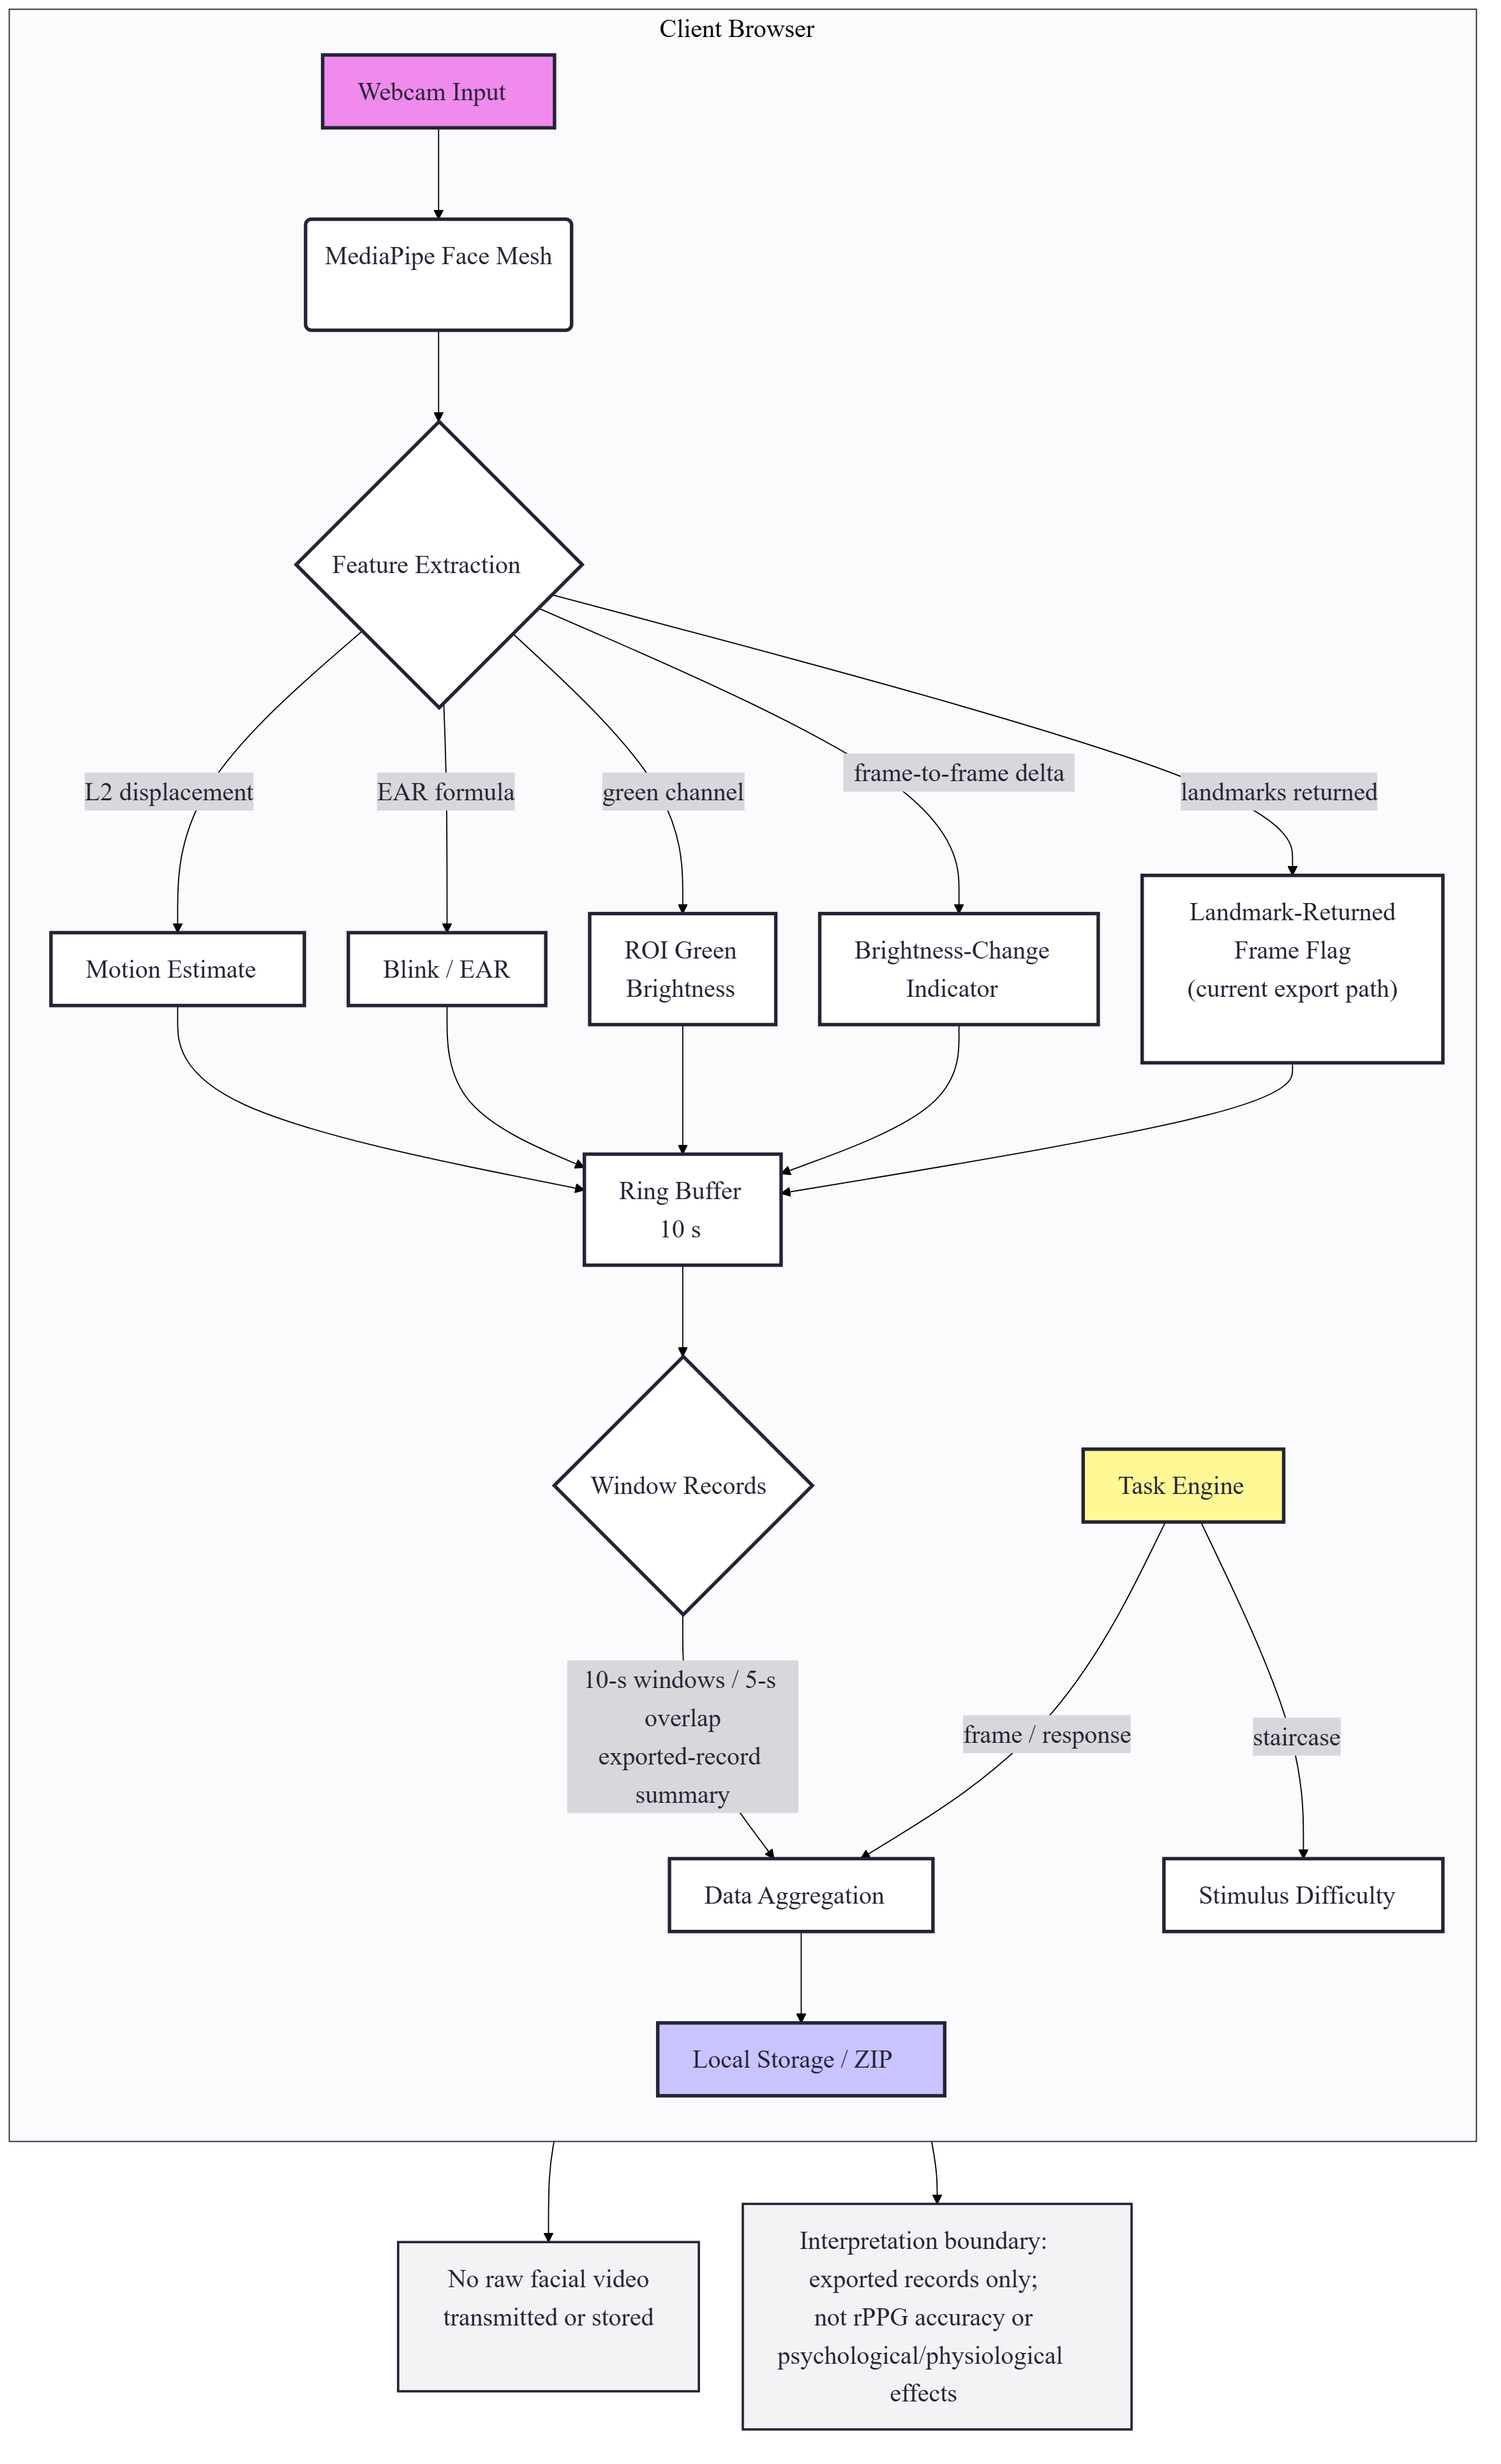
\includegraphics[width=.95\linewidth]{paper_figures/Figure1_SystemPipeline.png}
    \caption{Overview of the Camerala system architecture. The browser obtains webcam frames, extracts FaceMesh/rPPG-oriented features and quality indicators, synchronizes them with task events, and exports local logs. Under the tested implementation, only extracted features and task events are logged; raw video is neither transmitted nor stored by Camerala.}
    \label{fig:system_architecture}
\end{center}
\end{figure}

\subsection{High-Level Architecture}
The system enables a task-constrained experimental loop inside the browser sandbox (Fig. \ref{fig:system_architecture}).
The architecture consists of three coupled modules:
\begin{enumerate}
    \item \textbf{Task Engine}: Stimulus rendering, trial logic, key responses, feedback, staircase updates, and reaction-time logging.
    \item \textbf{Vision Pipeline}: Webcam ingestion, MediaPipe Face Mesh inference, rPPG-oriented ROI feature extraction, head-motion estimates, blink/EAR features, and frame-level quality indicators.
    \item \textbf{Data Manager}: Timestamp alignment, trial/frame aggregation, CSV serialization, ZIP packaging, and local persistence without raw-video storage.
\end{enumerate}

\subsection{Technical Implementation: The Vision Pipeline}
The current implementation uses MediaPipe Face Mesh, loaded through the browser, to obtain facial landmarks in real time.
The camera stream is requested through \texttt{getUserMedia} with ideal constraints of 640$\times$480 pixels and 30 fps.
Because actual camera settings can depend on the browser and device, these constraints should be interpreted as requested settings rather than verified hardware settings.

\subsubsection{Feature Extraction Logic}
The present implementation records sensor-derived features and quality indicators rather than validated clinical or medical measurements.
Two categories are central to this paper:

\textbf{1. Head Motion Index ($M_t$)}
Head motion is approximated from the frame-to-frame displacement of a facial landmark.
Let $L^t = (x^t, y^t)$ be the normalized landmark coordinate at frame $t$.
The motion scalar is computed as:
\begin{equation}
    M_t = || L^t - L^{t-1} ||_2 .
\end{equation}
This feature is used as a motion-related quality and behavior indicator.
It is not an algorithmic correction for motion artifacts in rPPG.

\textbf{2. ROI Brightness and Exposure Fluctuation ($E_{fluc}$)}
The implementation samples a small forehead region around a FaceMesh landmark and records the green-channel brightness as an rPPG-oriented ROI value.
It also computes a frame-level luminance-change indicator:
\begin{equation}
    E_{fluc}(t) = | Y_t - Y_{t-1} | ,
\end{equation}
where $Y_t$ is the downsampled frame-luminance average at frame $t$.
Camerala does not attempt to correct rPPG degradation caused by motion or illumination changes.
Instead, it records motion-related and luminance-related indicators so that data quality can be inspected and, if necessary, filtered during analysis.

\subsection{Technical Implementation: The Task Engine}
The experimental psychophysical probe is a two-alternative forced-choice orientation discrimination task.
Using the HTML5 Canvas API, the task engine procedurally renders oriented grating stimuli, records key responses, calculates reaction time with \texttt{performance.now()}, and updates task difficulty.
Procedural rendering avoids network-dependent stimulus loading during a trial and keeps task timing in the same browser runtime as feature logging.

\subsubsection{Timing and Synchronization}
The implementation uses the following timing strategy:
\begin{enumerate}
    \item \textbf{High-resolution timestamps}: Task events and frame features are timestamped using \texttt{performance.now()}.
    \item \textbf{Frame-loop alignment}: Feature extraction and task rendering are coordinated with the browser frame loop.
    \item \textbf{Local runtime alignment}: Task events and sensor-derived features are logged in the same browser runtime, avoiding server-side reconciliation.
\end{enumerate}

\begin{algorithm}
\caption{Camerala Task Loop (Simplified)}
\begin{algorithmic}
\STATE \textbf{Initialize} Camera, FaceMesh, Canvas
\WHILE{Session Active}
    \STATE $Block \leftarrow$ GetCurrentBlock()
    \STATE $Context \leftarrow Block.instruction$
    \STATE ShowInstruction(Context.text)
    \FOR{trial $i = 1$ to $n$}
        \STATE ShowFixation()
        \STATE $t_{onset} \leftarrow$ performance.now()
        \STATE DrawOrientationStimulus()
        \WHILE{No KeyPress}
            \STATE Poll Keyboard Input
        \ENDWHILE
        \STATE $t_{response} \leftarrow$ performance.now()
        \STATE $RT \leftarrow t_{response} - t_{onset}$
        \STATE LogTaskEvent($RT$, Accuracy, Context)
        \STATE LogFrameFeatures(FaceMeshFeatures, QualityIndicators)
    \ENDFOR
\ENDWHILE
\end{algorithmic}
\end{algorithm}

\subsection{Data Management and Local-First Persistence}
The current implementation uses JSZip to export local log files as a ZIP archive.
The archive contains \texttt{metadata.json}, \texttt{trials.csv}, \texttt{features\_raw.csv}, \texttt{windows.csv}, \texttt{blocks.csv}, and \texttt{subjective.csv}.
The metadata file stores the session ID, start time, user agent, and block plan.
The user initiates the download at the end of the session.
This design avoids Camerala-side raw-video storage and avoids raw-video transmission, but it also reduces the ability to inspect image artifacts retrospectively.
For this reason, Camerala logs quality indicators such as FPS, approximate face size, face-tracking availability, luminance, exposure fluctuation, and head motion.

% =================================================================================
% SECTION 4: METHODOLOGY
% =================================================================================
\section{Methodology}

\subsection{Target Usage Scenario and Exploratory Deployment}
The target usage scenario is a remote or home-based psychophysical task performed while seated in front of a laptop, with browser-based logging of behavioral events and webcam-derived features.
This is a task-constrained home/laboratory deployment, not continuous physiological sensing during ordinary daily activities such as walking, cooking, conversation, or night-time use.

To evaluate operational completion under this scenario, we conducted an exploratory longitudinal deployment with one author-participant.
The deployment consisted of 10 sessions and 600 total trials.
Each session consisted of six 10-trial blocks, with two blocks for each instructional task context (neutral instruction, negative instruction, and positive instruction), as reflected in the exported block plans.
The order of blocks was randomized by the web application.

\begin{figure*}[t]
    \begin{center}
    \fbox{\begin{minipage}{0.90\textwidth}
    \textbf{Descriptive longitudinal view of head-motion estimates}\\[1mm]
    laboratory \hfill home\\
    \rule{0.43\textwidth}{0.4pt}\textbar\rule{0.43\textwidth}{0.4pt}\\
    Window order over 10 sessions; instructional task contexts: neutral instruction, negative instruction, and positive instruction.\\
    \textit{Descriptive trend only; no psychological or physiological response label is used.}
    \end{minipage}}
    \caption{Descriptive longitudinal view of head-motion estimates over the 10-session deployment. The schematic emphasizes the descriptive organization of aggregated windows by session time, instructional task context, and laboratory/home context. The divider separates the laboratory and home portions of the available dataset. The figure is descriptive and should not be interpreted as evidence of a psychological or physiological effect.}
    \label{fig:longitudinal_motion}
\end{center}
\end{figure*}

\subsection{Participant (Autoethnography)}
The participant was the primary author.
This was a self-experimentation evaluation: no other participants were involved, no identifiable raw video was transmitted by Camerala, and the author provided informed consent for self-participation.
Because the participant was also the author and knew that the task instructions were experimental, the instruction blocks cannot be assumed to have induced evaluation pressure, reward motivation, or psychological effects.
They are used only as different instructional task contexts for demonstrating synchronized logging across task conditions.

\subsection{Hardware and Software Configuration}
Table \ref{tab:hardware_config} reports the hardware/software information available for the deployment.
Unknown or unrecorded deployment-time details are explicitly marked rather than inferred from the current revision environment.

\begin{table*}[t]
\caption{Hardware and software configuration}
\label{tab:hardware_config}
\begin{center}
\small
\begin{tabular}{p{0.28\textwidth}p{0.64\textwidth}}
\toprule
\textbf{Item} & \textbf{Reported value} \\
\midrule
Laptop/PC model & Not logged \\
CPU & Not logged \\
GPU & Not logged \\
RAM & Not logged \\
Operating system & Available logs report Windows NT 10.0 in the browser user agent; exact OS build/version not logged \\
Browsers used & Mozilla Firefox and Google Chrome were used according to author-provided information. Available exported metadata records Firefox user agents for the sessions in the repository; Chrome deployment-time version is not logged. \\
Recorded Firefox user agent & \texttt{Mozilla/5.0 (Windows NT 10.0; Win64; x64; rv:147.0) Gecko/20100101 Firefox/147.0} in available session metadata. \\
Webcam type/model & Not logged \\
Requested camera constraints & \texttt{getUserMedia}: ideal 640$\times$480 pixels, ideal 30 fps. \\
Actual camera resolution & Not programmatically logged. \\
Actual camera frame rate & Not programmatically logged; measured processing FPS is reported in Table \ref{tab:data_quality}. \\
Display refresh rate & Approximately 60 Hz target refresh rate. \\
Viewing distance & Approximately 50--60 cm. \\
Auto-exposure & Device/browser default; exact deployment-time state not programmatically logged. \\
Auto-white-balance & Device/browser default; exact deployment-time state not programmatically logged. \\
\bottomrule
\end{tabular}
\end{center}
\end{table*}

\subsection{Deployment Environment and Lighting Conditions}
Ambient illuminance was estimated at the participant's eye level.
The reported lux values summarize the available deployment notes, but the exact measurement window and lux meter model require author confirmation.
Table \ref{tab:environment_config} separates reported facts from information that was not systematically recorded.

\begin{table*}[t]
\caption{Deployment environment and lighting conditions}
\label{tab:environment_config}
\begin{center}
\small
\begin{tabular}{p{0.24\textwidth}p{0.32\textwidth}p{0.32\textwidth}}
\toprule
\textbf{Item} & \textbf{Laboratory} & \textbf{Home} \\
\midrule
Ambient illuminance & $480 \pm 20$ lux & $140 \pm 50$ lux \\
Lux meter model & \multicolumn{2}{p{0.64\textwidth}}{Not logged} \\
Lux meter position & Eye level of participant & Eye level of participant \\
Lux measurement timing/window & \multicolumn{2}{p{0.64\textwidth}}{Not systematically recorded} \\
Window presence & Not systematically recorded & Not systematically recorded \\
Natural light contribution & Not systematically recorded & Not systematically recorded \\
Artificial lighting & Standard fluorescent lighting & Mixed LED and monitor glow \\
Time of day & Not systematically recorded & Not systematically recorded \\
Weather & Not systematically recorded & Not systematically recorded \\
Curtain/blind condition & Not systematically recorded & Not systematically recorded \\
Screen brightness setting & \multicolumn{2}{p{0.64\textwidth}}{Not systematically recorded} \\
Mean luminance aggregation & \multicolumn{2}{p{0.64\textwidth}}{Computed from exported frame/window logs; implementation uses 10-s windows with 5-s overlap for aggregated windows.} \\
Exposure fluctuation aggregation & \multicolumn{2}{p{0.64\textwidth}}{Frame-level absolute luminance difference, summarized in 10-s windows with 5-s overlap.} \\
Clouds/screen flicker/power cycles & \multicolumn{2}{p{0.64\textwidth}}{Possible sources of luminance fluctuation; not systematically recorded as observed events in each session.} \\
\bottomrule
\end{tabular}
\end{center}
\end{table*}

\subsection{Experimental Procedure and Instructional Task Contexts}
Each session began with a pre-session capture check for basic camera conditions, including approximate luminance, pose, and face size, before the camera feed was hidden to reduce distraction.
Before each block, the system presented one of three instructional task contexts: neutral instruction, negative instruction, or positive instruction.
The negative and positive instruction blocks were not interpreted as validated cognitive or motivational manipulations.
They were used to demonstrate that Camerala can synchronize behavioral logs and sensor-derived features across different task contexts.

\subsection{Psychophysical Task}
The task was an orientation discrimination task.
Each trial consisted of a fixation period, a brief oriented stimulus, a response window, and immediate visual feedback.
The application recorded stimulus/task events, responses, reaction time, correctness, and task difficulty together with frame-level sensor-derived features.

\subsection{Dependent Measures and Pre-processing}
All exported logs were processed sequentially.
The primary behavioral measure was reaction time (RT), with an operational analysis range of 100--1500 ms.
The primary sensor-derived and quality measures were FPS, face size, face-tracking availability/quality, mean luminance, exposure fluctuation, head motion, and rPPG-oriented ROI brightness.
Trials outside the RT range and records below the operational face-tracking threshold were excluded.
The threshold of 0.8 was used as an operational exclusion threshold in the exploratory analysis to remove records with low FaceMesh tracking confidence. This threshold was not independently validated as an rPPG-quality threshold; therefore, the resulting face-tracking availability is treated only as a FaceMesh/logging quality indicator. It does not directly validate rPPG signal quality or landmark accuracy.

% =================================================================================
% SECTION 5: RESULTS
% =================================================================================
\section{Results}

The results are reported descriptively as sensor-derived observations under the tested configuration.
The deployment completed 10 sessions, 30 instructional-context groups, and 600 total trials, and the exported local logs were available for analysis.
After applying the operational RT and face-tracking exclusion criteria, 582 trials were retained (97.0\% retention).
This retention rate describes the available analyzed records under the tested configuration and does not demonstrate broad operational generality across devices, users, or environments.

\subsection{Measurement-Quality Indicators}
Table \ref{tab:data_quality} and Fig. \ref{fig:data_quality} summarize measurement-quality indicators in the laboratory and home contexts.
The home context showed lower mean luminance and higher exposure fluctuation in the exported logs.
After filtering, FaceMesh tracking did not substantially fail under the tested configuration. This indicator should be read only as a FaceMesh/logging quality indicator, not as validation of rPPG quality.

\begin{figure}[t]
    \begin{center}
    \fbox{\begin{minipage}{0.82\linewidth}
    \textbf{Exposure fluctuation by context}\\[1mm]
    laboratory: lower exported window-level exposure fluctuation\\
    home: higher exported window-level exposure fluctuation\\
    \textit{Descriptive measurement-quality indicator only.}
    \end{minipage}}
    \caption{Descriptive comparison of exposure fluctuation by deployment context. The schematic summarizes exported window-level exposure fluctuation values; higher values indicate greater frame-to-frame luminance variation. The figure does not show face-tracking availability.}
    \label{fig:data_quality}
\end{center}
\end{figure}

\begin{table*}[t!]
    \caption{Descriptive measurement-quality comparison}
\label{tab:data_quality}
\begin{center}
\small
\begin{tabular}{lcc}
\toprule
\textbf{Metric (Mean $\pm$ SD unless noted)} & \textbf{Laboratory (292 trials)} & \textbf{Home (290 trials)} \\
\midrule
Measured processing FPS & $59.8 \pm 0.4$ & $58.2 \pm 2.1$ \\
Face size (IOD in px) & $142 \pm 12$ & $135 \pm 18$ \\
Mean luminance ($Y$) & $180 \pm 15$ & $110 \pm 45$ \\
Exposure fluctuation ($E_{fluc}$) & $0.03 \pm 0.01$ & $0.09 \pm 0.04$ \\
Face-tracking availability after filtering & $99.1\%$ & $96.5\%$ \\
\bottomrule
\end{tabular}
\end{center}
\end{table*}

\subsection{Task-Event and Sensor-Derived Observations}
To address RQ2, we compared descriptive task-event and sensor-derived summaries across instructional task contexts and deployment contexts.
Figure \ref{fig:rt_results} shows descriptive differences in head-motion estimates and RT across laboratory and home contexts.
The plotted differences should be interpreted as observations from this author-participant deployment, not as evidence that the instruction blocks induced psychological or motivational effects.

\begin{figure*}[t]
    \begin{center}
    \fbox{\begin{minipage}{0.90\textwidth}
    \textbf{Panel A: Head-motion estimates}\hfill \textbf{Panel B: Reaction time}\\[1mm]
    Conditions: neutral instruction, negative instruction, positive instruction.\\
    Contexts: laboratory and home.\\
    \textit{No p-values, significance marks, or psychological/physiological effect labels are shown.}
    \end{minipage}}
    \caption{Descriptive task-event and sensor-derived summaries by context. Panel A shows head-motion estimates; Panel B shows reaction time. Conditions refer to instructional task contexts. The trends are descriptive and do not validate physiological, cognitive, or motivational effects.}
    \label{fig:rt_results}
\end{center}
\end{figure*}

In the laboratory context, the negative instruction block showed a lower mean RT than the neutral block in this dataset.
In the home context, the mean RT values across instruction blocks were closer together.
Because the deployment used one author-participant and did not isolate instruction effects from environment, lighting, posture, or camera factors, these RT patterns are reported only as descriptive task-event observations.

\subsection{rPPG-Oriented ROI Estimates}
The exported data include rPPG-oriented ROI brightness values and related quality indicators, but no ECG or contact PPG reference was collected.
Therefore, the manuscript does not interpret block-level ROI-derived differences as validated heart-rate changes.
Because no ECG or contact PPG reference was collected, block-level bpm-style summaries are not interpreted as validated heart-rate changes in this paper. The appropriate interpretation is that the tested deployment yielded sensor-derived estimates and quality indicators whose values differed descriptively between the tested laboratory and home contexts.

% =================================================================================
% SECTION 6: DISCUSSION
% =================================================================================
\section{Discussion}

The main implication of this revision is system-design oriented.
Camerala illustrates how a browser-native runtime can combine task events, webcam-derived features, quality indicators, and local persistence without raw-video transmission in a task-constrained home/laboratory setting.
The results do not establish general deployability, cross-device stability, or physiological or cognitive effects.
Instead, they motivate design requirements and safeguards for future local-first deployments.

\subsection{Browser-Native Local-First Logging as a Design Pattern}
The useful system property demonstrated here is integration.
Task timing, frame-level feature extraction, quality indicators, and local export are handled in one client-side workflow.
This can reduce the need for raw-video handling and server-side timestamp reconciliation.
However, because raw video is not stored, researchers lose the ability to visually inspect many artifacts after data collection.
This trade-off makes quality-aware logging especially important.

\subsection{Quality Indicators for Task-Constrained Home/Laboratory Deployment}
The deployment suggests that future systems should log not only task performance and rPPG-oriented estimates, but also indicators that help interpret the measurement pipeline.
Such indicators include FPS, face size, face-tracking availability, luminance, exposure fluctuation, and head motion.
These values can support pre-session checks, quality flags, and quality-gated analysis.
They should not be treated as proof that rPPG estimates are accurate.

\subsection{Interpreting Sensor-Derived Estimates Under Environmental Heterogeneity}
The home and laboratory contexts differed in illumination and exposure fluctuation in the available logs.
Because lighting, posture, camera placement, screen luminance, and task context were not independently controlled, the observed differences cannot be attributed to psychological or physiological state.
They are better understood as deployment-specific sensor-derived observations under environmental heterogeneity.
Future work should include reference ECG or contact PPG, multiple participants, multiple devices, and controlled variation of environmental factors.

\subsection{Design Safeguards for Future Camerala Deployments}
Future deployments should incorporate clearer safeguards: documented hardware/browser/camera settings, explicit reporting of camera constraints and actual camera settings, pre-session lighting checks, face-size and tracking warnings, luminance and exposure-fluctuation flags, and predefined quality-gated analysis rules.
If privacy-sensitive raw video is not stored, these safeguards become more important because many artifacts cannot be retrospectively inspected from images.
For studies that aim to make claims about physiological responses, a reference physiological sensor and a multi-participant design are necessary.

\subsection{Limitations}
This study has strict limitations.
First, it was an exploratory N=1 deployment with the author as participant.
Second, there was no reference physiological sensor, ECG, or contact PPG.
Third, the deployment used one primary laptop/camera configuration and did not test multiple devices, multiple participants, or multiple home environments.
Fourth, lighting, posture, camera placement, and task context were not experimentally separated.
Fifth, no comparison with existing experiment runtimes, browser rPPG tools, or cloud APIs was conducted.
Sixth, the study does not claim clinical or medical accuracy, general deployability, broad operational generality, cross-device stability, or validated cognitive, motivational, psychological, or physiological effects.
The present study presents an implementation example of browser-native, task-aligned, local-first feature logging under limited home/laboratory conditions.

\section{Conclusion}
We presented Camerala, a browser-native, local-first framework that integrates psychophysical task execution, on-device rPPG/FaceMesh-derived feature extraction, measurement-quality indicators, and timestamped local persistence.
In a limited 10-session N=1 author-participant deployment across one laboratory setting and one home setting, the system completed data collection under the tested configuration without raw video transmission by Camerala.
The deployment produced synchronized behavioral logs, sensor-derived features, and quality indicators, and it revealed descriptive differences between the tested environments.
These observations should not be interpreted as evidence of general deployability, cross-device stability, or physiological or cognitive effects.
Instead, Camerala illustrates a task-aligned browser-native implementation and highlights design safeguards needed for future local-first physiological feature logging in home-based psychophysical experiments.

\section*{Data availability}
The dataset containing facial landmarks, sensor-derived features, and behavioral responses associated with this study cannot be made publicly available due to privacy restrictions and potentially identifiable face-derived data from a domestic deployment context.

\section*{CRediT authorship contribution statement}
\textbf{Kotaro Furukawa}: Conceptualization, Methodology, Software, Investigation, Formal analysis, Writing - original draft.

\section*{Declaration of competing interest}
The author declares that there are no known competing financial interests or personal relationships that could have appeared to influence this work.

\section*{Funding}
This work was supported by the College of Transdisciplinary Sciences for Innovation, Kanazawa University.

\section*{Declaration of generative AI and AI-assisted technologies in the manuscript preparation process}
During the preparation and revision of this manuscript, the author used generative AI tools, including Google Gemini and OpenAI Codex/ChatGPT, to assist with LaTeX formatting, wording refinement, and response-draft preparation. The author reviewed and edited the content and takes full responsibility for the manuscript.



\begin{thebibliography}{99}

\bibitem{verkruysse2008}
Wim Verkruysse, Lars~O. Svaasand, and J. Stuart Nelson.
\newblock Remote plethysmographic imaging using ambient light.
\newblock {\em Optics Express}, 16(26):21434--21445, 2008.

\bibitem{poh_ica}
Ming-Zher Poh, Daniel~J. McDuff, and Rosalind~W. Picard.
\newblock Non-contact, automated cardiac pulse measurements using video imaging and blind source separation.
\newblock {\em Optics Express}, 18(10):10762--10774, 2010.

\bibitem{deepphys}
Weixuan Chen and Daniel McDuff.
\newblock Deepphys: Video-based physiological measurement using convolutional attention networks.
\newblock In {\em Proceedings of the European Conference on Computer Vision (ECCV)}, pages 349--365, 2018.

\bibitem{gupta_etemad_2023}
Divij Gupta and Ali Etemad.
\newblock Privacy-preserving remote heart rate estimation from facial videos.
\newblock In {\em BMVC 2023 Workshop Proceedings}, 2023.

\bibitem{ayesha2022_web}
Amtul Haq Ayesha, Donghao Qiao, and Farhana Zulkernine.
\newblock A web application for experimenting and validating remote measurement of vital signs.
\newblock In {\em Proceedings of the 20th International Conference on Smart Homes and Health Telematics}, pages 256--267, 2022.

\bibitem{dilernia2024}
Daniele Di Lernia, Gianluca Finotti, Manos Tsakiris, Giuseppe Riva, and Marnix Naber.
\newblock Remote photoplethysmography (rPPG) in the wild: Remote heart rate imaging via online webcams.
\newblock {\em Behavior Research Methods}, 56(7):6904--6914, 2024.

\bibitem{labvanced_rppg}
LabVanced.
\newblock Remote heart rate detection / rPPG technology page.
\newblock Public online system documentation, accessed during manuscript revision.

\bibitem{facephys_demo}
Kegang Wang and contributors.
\newblock FacePhys-Demo: Browser-based remote photoplethysmography monitor.
\newblock Public software demonstration repository, accessed during manuscript revision.

\bibitem{rhythmedge}
Mohammad A. Al Faruque and colleagues.
\newblock RhythmEdge: Enabling contactless heart rate estimation on the edge.
\newblock In {\em IEEE International Conference on Smart Computing}, 2022.

\end{thebibliography}

\appendix{}
\subsection*{Supporting Example: Task Substitution}

A core engineering feature of the framework is the separation between task logic and the feature-extraction loop.
Listing 1 illustrates a simplified configuration for replacing the orientation task with a spatial-memory task while preserving the same logging pathway.
This example is intended to illustrate module separation rather than to provide additional validation data.

\vspace{3mm}
\noindent\footnotesize{\textbf{Listing 1:} Task substitution example}
\vspace{-1mm}
\begin{lstlisting}[basicstyle=\ttfamily\scriptsize, frame=single, language=JavaScript]
const task = {
  stimulus: renderSpatialGrid(memory_load_target),
  allowed_keys: ["Space"],
  on_frame_sync: (timestamp_ms) => {
    camerala_logger.logEvent("stimulus_onset", timestamp_ms);
  }
};
\end{lstlisting}
\vspace{2mm}

Listing 2 shows a schema-style example of a local tabular log in which task events and frame-derived features can coexist through timestamps.

\vspace{3mm}
\noindent\footnotesize{\textbf{Listing 2:} Example local log schema}
\vspace{-1mm}
\begin{lstlisting}[basicstyle=\ttfamily\tiny, frame=single, language=csv]
time_ms,event,load,rppg_roi,head_motion
4015.2,grid_on,4,110.4,0.02
4016.8,frame_sync,4,109.8,0.02
4032.5,frame_sync,4,111.1,0.01
4211.4,response,4,112.0,0.01
\end{lstlisting}
\vspace{2mm}

\end{document}
